% !TEX program = xelatex
\documentclass{resume} % 简历文档类（自带图标、datedsubsection等基础命令）

% 1. 仅保留必要宏包（删除冲突项，避免重复加载）
\usepackage{graphicx}               % 图片插入（必选）
\usepackage{zh_CN-Adobefonts_external} % 中文Adobe字体（必选，确保中文显示）
\usepackage{url}                    % URL格式支持（必选）
\usepackage{geometry}               % 页边距调整（必选）
\usepackage{xcolor}                 % 颜色定义（仅加载1次，解决darkgreen未定义）
\usepackage{hyperref}               % 链接功能（最后加载，避免冲突）

% 2. 页边距配置（适配文本宽度，减少Overfull）
\geometry{top=0.8cm, bottom=1.5cm, left=1.4cm, right=1.4cm} % 左右边距各减0.1cm，避免超宽

% 3. 颜色与链接配置（保持原风格，兼容打印）
\definecolor{darkgreen}{RGB}{0, 100, 0} % 定义深绿色
\hypersetup{
	colorlinks=true,
	linkcolor=blue,
	urlcolor=darkgreen,
	breaklinks=true,
	unicode=true,
	pdfstartview=FitH
}

% 4. 重新定义“稍粗+深色”样式（颜色调深，粗细可按需调整）
% 颜色：gray!50（比原来的gray!70深很多）
% 粗细：\bfseries（粗体）+ 11pt字号（比原来的10.5pt稍大，更突出）
\newcommand{\highlight}[1]{{\bfseries\fontsize{13pt}{13pt}\selectfont\textcolor{gray!90}{#1}}}

\begin{document}
	\pagenumbering{gobble} % 隐藏页码
	
	% 个人信息区（保持原布局，无修改）
	\vspace*{-10pt}
	\noindent
	\begin{tabular}{@{}p{0.64\textwidth}@{\hspace{0.02\textwidth}}p{0.34\textwidth}@{}}
		\centering
		\LARGE\bfseries 张建\\[6pt]
		\normalsize
		求职意向：Agent开发工程师 / 大模型应用开发 / AI 智能体工程师\\[3pt]
		个人网站：\href{https://husterzj.info/}{\textcolor{black}{HUSTERZJ.INFO}}\\[3pt]
		\faEnvelope\ m202473806@hust.edu.cn\\[3pt]
		\faPhone\ 15237776378 \hspace{1em} \faCalendar\ 25岁
		&
		\raggedleft
		\vspace{-30pt}
		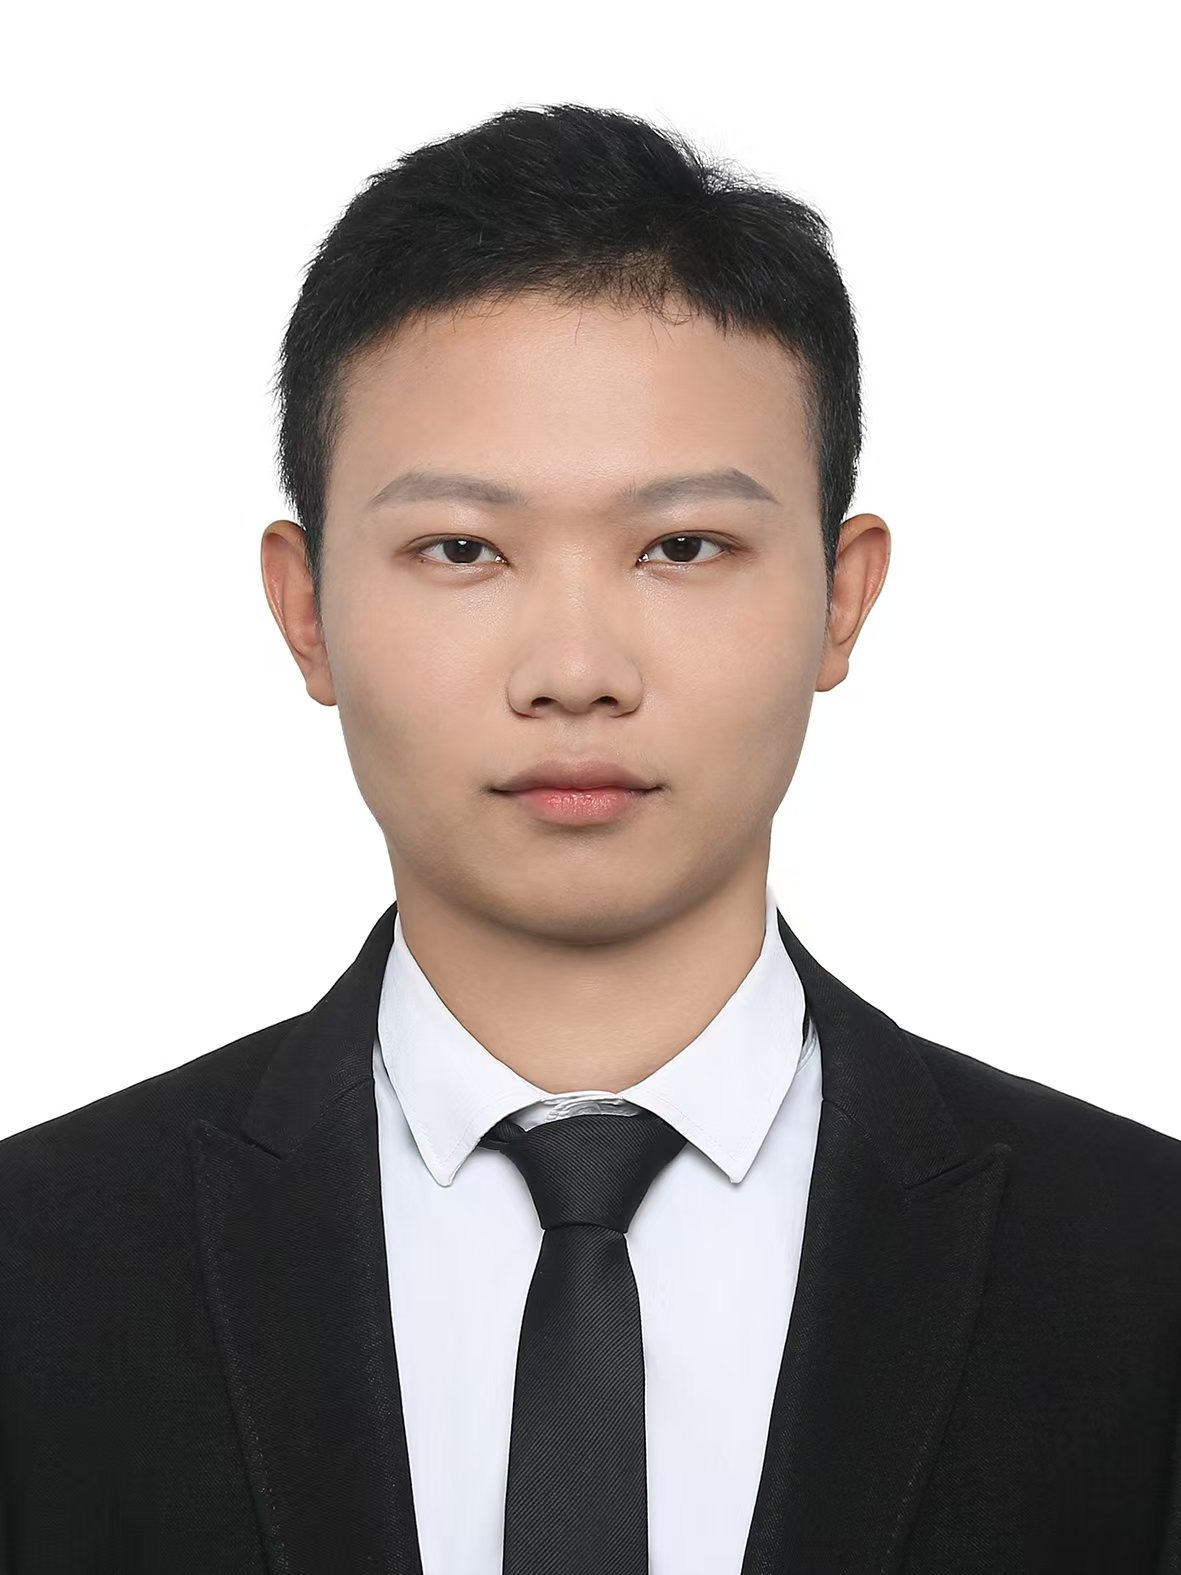
\includegraphics[width=1.05in]{zj} % 确保图片文件“zj”在当前目录（如zj.jpg/png）
	\end{tabular}
	\vspace{-5pt}
	
	\section{\faCog\ 专业技能}
	\begin{itemize}[parsep=0.5ex] % 紧凑列表，避免冗余
		\item AI智能体开发：熟悉 ReAct、Plan-and-Solve、Reflection 等 Agent 决策范式；了解 LangChain、AutoGen、Openclaw 等框架；了解多智能体协同、向量数据库、Embedding技术；尝试过模型微调
		\item Agent工程落地：熟悉 Coze、Dify、n8n 等低代码编排平台；具备 Agent Skills 设计、工具集成、流程编排与系统部署能力
		\item 全栈开发：熟练使用 Python；掌握 Vue3 前端开发 以及 FastAPI/Django 后端开发；熟悉 Git，有扎实的数据结构和算法基础
		\item AI 工具链：精通 Cursor/ClaudeCode AI 编码；能独立完成需求分析、原型设计（Figma/Axure/ 墨刀）与项目文档沉淀
		\item 协作与交付：具备需求拆解、跨角色协同、项目推动与从 0→1 落地能力

	\end{itemize}
	
	\section{\faGraduationCap\ 教育经历}
	\datedsubsection{\textbf{华中科技大学} \hspace{1em} \textit{人工智能与自动化学院 - 智能科学与技术学硕}}{2024.9 -- 至今}
	主修课程：智能计算系统、机器人导论、现代最优化理论与方法等
	
	\datedsubsection{\textbf{华中科技大学} \hspace{1em} \textit{人工智能与自动化学院 - 自动化专业工学学士}}{2019.9 -- 2024.6}
	专业排名前5\%。主修课程：模式识别、计算机网络、数据结构、C语言、数据库等
	
	\section{\faBriefcase\ 项目经历}
	% 减小hspace间距（从3em→2em），解决Overfull \hbox
	
	\datedsubsection{\textbf{基于多智能体协同的智能旅行助手系统} \hspace{1em} \textit{个人实践项目 \hspace{2em}
			\href{http://ideas-test.com/}{http://ideas-test.com/}}}{2026.4 -- 2026.5}
	\large {技术栈：Python \textbullet{} FastAPI \textbullet{} Vue3 \textbullet{} LLM Agent \textbullet{} Tool Use
		\textbullet{} 高德地图API}
	\begin{itemize}
	    \item{多智能体架构设计}：设计4个功能Agent（景点搜索/天气查询/酒店推荐/行程规划），各Agent配备专项Prompt与
		共享MCP工具集，实现职责分离与协同规划。
		\item {工具调用与数据集成}：集成高德地图API、天气服务等外部数据源，基于Tool Use模式实现动态信息获取与行程生成。
		\item {Prompt工程}：针对各Agent设计结构化System Prompt与Few-shot示例，引导LLM生成准确的工具调用与行程规划结果。
		\item {预算自动核算}：基于住宿等级、交通方式、景点门票自动计算费用明细，生成完整预算报告。
		\item {全栈交付与部署上线}：基于 FastAPI 提供后端 RESTful 服务，Vue3 集成高德地图实现路线可视化与点位标注；使用阿里云 ECS + 域名完成上线，通过 Nginx 反向代理实现前后端高效联调与稳定访问。
	\end{itemize}
	
	\datedsubsection{\textbf{航天器任务调度原型系统开发} \hspace{1em} \textit{国自然重点项目 \hspace{2em} \href{https://astroscheduler.cn/}{https://astroscheduler.cn/}}}{2024.5 -- 2025.10}
	\large {技术栈：Python \textbullet{} FastAPI \textbullet{} Vue3 \textbullet{} TypeScript \textbullet{} Pinia}
	\begin{itemize}
		\item 开源项目地址：\href{https://gitee.com/husterzj/spacetaskscheduler}{\textcolor{darkgreen}{https://gitee.com/husterzj/spacetaskscheduler}}
		\item 复杂业务建模与通用化架构设计：面对高度耦合、充满不确定性的航天调度场景，主导需求分析与领域建模，打通业务壁垒，将依赖人工经验的调度流程抽象为规划包管理、资源管理、任务管理、算法配置、结果生成5大标准化模块，基于清晰的通用化业务边界完成架构设计，支撑未来任务的可扩展接入
		\item 外部工具封装与标准化调用：将Java启发式调度算法封装为标准化服务接口，设计JSON Schema输入输出协议，通
		过subprocess实现跨语言工具调用与结果解析，支持异步执行与异常回退
		\item 多阶段工作流编排：设计并实现数据转换、约束预处理、算法调度、结果可视化的Pipeline API，基于Pydantic定义各阶段数据契约与状态流转机制，保障复杂任务链的可靠执行与错误隔离
		\item 全栈工程化与部署上线：基于Vue3+TypeScript开发交互式配置界面，使用Pinia设计模块化状态管理，集成dhtml
		x-gantt实现资源/任务多维度甘特图可视化；独立完成前后端分离架构设计与生产环境部署（Nginx + Linux Screen）
		\item LLM-Agent技术预研：规划系统v2.0智能化升级路径，设计基于大模型的冲突检测与消解方案——利用LLM解析调度
		结果中的资源冲突与约束违反，结合领域知识生成可执行消解建议；预研自然语言驱动的任务配置生成与外部求解器（CPLEX/COPT）Tool-use调用链路
	\end{itemize}
	
	
	\section{\faUser\ 自我评价}
	\hspace{2em}深耕 AI 与智能系统领域，保持对前沿技术的高度敏锐与自驱学习。极具极客精神与强落地能力，累计持有 12 个域名（其中 4 个已备案），先后独立运维十余台服务器开展项目全生命周期部署与环境搭建。
	
	\hspace{2em}作为 ENFJ 型人格，我酷爱思考与总结，不断从学习实践中提炼属于自己的理论方法，有着很强的分享欲和表达欲。以下是我自己梳理的常用的资源地图：
	\begin{itemize}[parsep=0.5ex, leftmargin=1.5em]
	    \item 软件相关实用网址：\href{https://roadmap.sh/r/rdm-xqyvk}{\textcolor{darkgreen}{https://roadmap.sh/r/rdm-xqyvk}}
	    \item 硬件相关实用网址：\href{https://roadmap.sh/r/copy-lsiu7}{\textcolor{darkgreen}{https://roadmap.sh/r/copy-lsiu7}}
	\end{itemize}

	\section{\faTrophy\ 荣誉及证书}
	\begin{itemize}
		\item 奖项：“中国软件杯” 大学生软件设计大赛决赛三等奖、蓝桥杯Python三等奖、“西门子杯”信息化网络化赛道华中赛区三等奖
		\item 荣誉：优秀毕业生、优秀学生干部、一等硕士学业奖学金、海信奖学金、金毓岗陆兰英奖学金、自强奖学金、学习优秀奖学金
		\item 证书：计算机三级网络技术、 CET-6、MBSE（理论、实践与软件）高级证书
		\item 学生工作：弄潮社（社团）副会长、学习委员、MBA班级AI实操课程代理讲师（150+同学）
	\end{itemize}
	
	\section{\faFileImageO\ 附件 - 相关页面}
	\begin{center}
		% 第一张图：航天器任务调度原型系统
		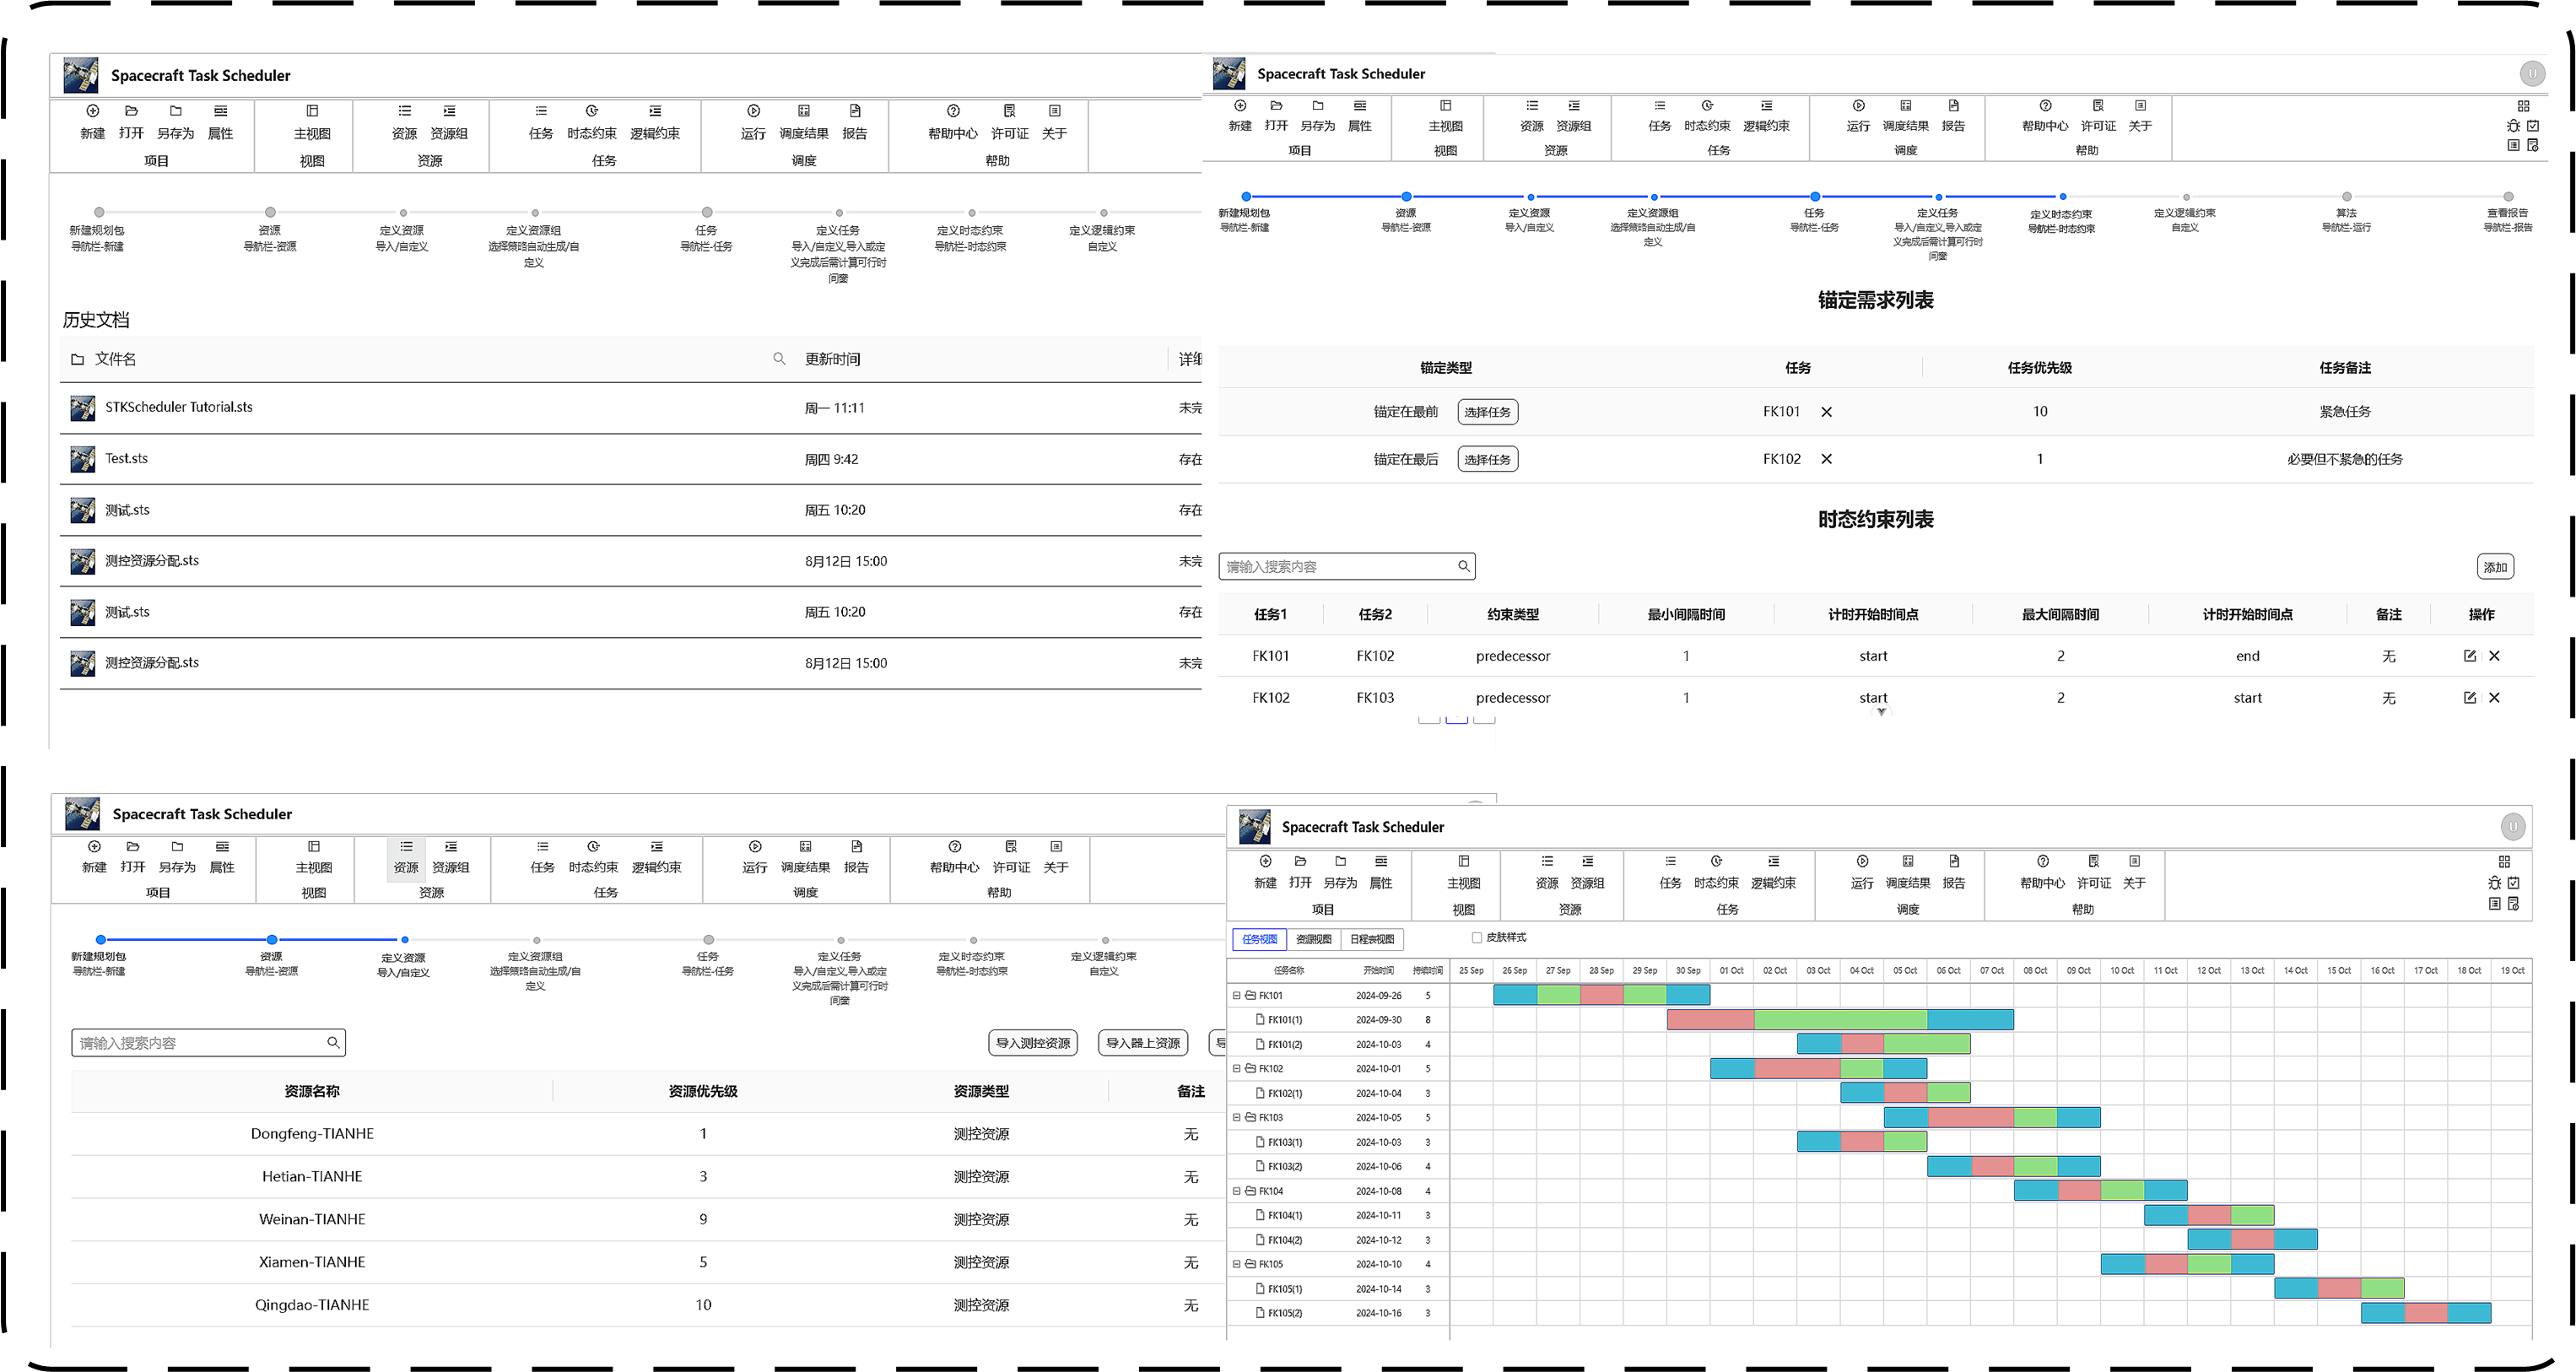
\includegraphics[width=1\textwidth]{fujian/7_航天器任务调度原型系统.png} \\[5pt]
		\small\centering 航天器任务调度原型系统 \\[15pt] % 图下方说明文字，加15pt间距分隔两张图
		
	\end{center}
	
\end{document}